\def\mytitle{PARALLELOGRAM}
\def\myauthor{VUNNAVA SRAVANI}
\def\contact{sravani21vunnava@gmail.com}
\def\mymodule{Future Wireless Communication (FWC)}
\documentclass[10pt, a4paper]{article}
\usepackage[a4paper,outer=1.5cm,inner=1.5cm,top=1.75cm,bottom=1.5cm]{geometry}
\twocolumn
\usepackage{setspace}
\usepackage{graphicx}
\graphicspath{{./images/}}
\usepackage[colorlinks,linkcolor={black},citecolor={blue!80!black},urlcolor={blue!80!black}]{hyperref}
\usepackage[parfill]{parskip}
\usepackage{lmodern}
\usepackage{tikz}
	\usepackage{physics}
%\documentclass[tikz, border=2mm]{standalone}
\usepackage{karnaugh-map}
\usepackage{tabularx}
\usetikzlibrary{calc}
\usepackage{amsmath}
\usepackage{amssymb}
\renewcommand*\familydefault{\sfdefault}
\usepackage{watermark}
\usepackage{lipsum}
\usepackage{xcolor}
\usepackage{listings}
\usepackage{float}
\usepackage{titlesec}
\providecommand{\mtx}[1]{\mathbf{#1}}
\titlespacing{\subsection}{1pt}{\parskip}{3pt}
\titlespacing{\subsubsection}{0pt}{\parskip}{-\parskip}
\titlespacing{\paragraph}{0pt}{\parskip}{\parskip}
\newcommand{\figuremacro}[5]{//
    \begin{figure}[#1]
        \centering
        \includegraphics[width=#5\columnwidth]{#2}
        \caption[#3]{\textbf{#3}#4}
        \label{fig:#2}
    \end{figure}
}
\newcommand{\myvec}[1]{\ensuremath{\begin{pmatrix}#1\end{pmatrix}}}
\let\vec\mathbf
\lstset{
frame=single, 
breaklines=true,
columns=fullflexible
}

\title{\mytitle}
\author{\myauthor\hspace{1em}\\\contact\\FWC22012\hspace{6.5em}IITH\hspace{0.5em}\mymodule\hspace{6em}ASSIGN-5}
\date{}
\begin{document}
	\maketitle
	\tableofcontents

	\section{Construction}
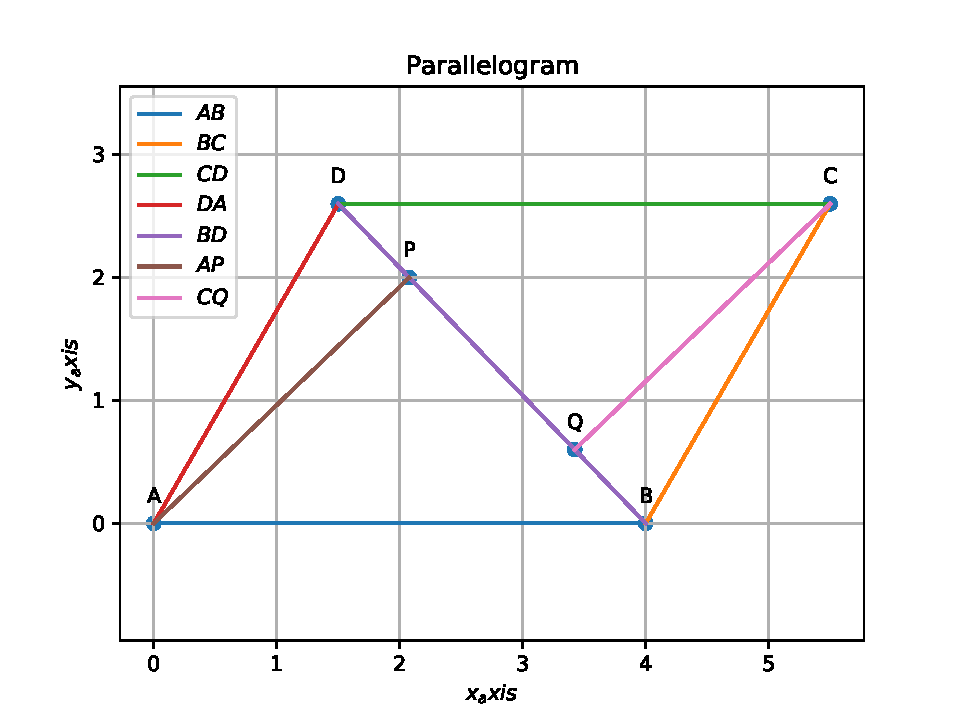
\includegraphics[scale=0.5]{matrixline.pdf}
   \section{Problem}
  ABCD is a parallelogram and AP and CQ are
perpendiculars from vertices A and C on diagonal
BD . Show that \\
(i) $\Delta APB \cong \Delta CQD$  \\       
(ii) AP = CQ

   \section{Solution}
\subsection{Considerations}
The input parameters for this construction are 
\begin{center}
\begin{tabular}{|c|c|c|}
	\hline
	\textbf{Symbol}&\textbf{Value}&\textbf{Description}\\
	\hline
	b&6&length of AB\\
	\hline
	r&5&length of AC\\
	\hline
	$\theta$&$\frac{\pi}{3}$&angle of parallelogram\\
	\hline
\end{tabular}\\
$\vec{A},\vec{B},\vec{C},\vec{D}$ are the coordinates of the parallelogram
\begin{center}
$\vec{A}=\myvec{0\\0}$
$\vec{D}=\myvec{r\cos\theta \\ r\sin\theta}$
$\vec{B}=\myvec{0\\b}$
$\vec{C} = \vec{B}+\vec{C}$
\end{center}
\end{center}
\subsection{Part 1}
	\textbf{To Prove: AP = CQ}

		
		The line equation for diagonal BD is
		\begin{center}
   		\begin{equation}
		x = \vec{B}+\lambda\vec{m}
		\end{equation}
		
		\begin{equation}
		\vec{m} = \vec{B}-\vec{D}
		\end{equation}
			$\vec{P} , \vec{Q}$ are foot of perpendiculars drawn from A and C on to the diagonal BD
		\begin{equation}
		\vec{P} = \vec{B} - \frac{\vec{m}^T \vec{B}}{\norm{\vec{m}}^2}\vec{m}
		\end{equation}
		\begin{equation}
		\vec{Q} = \vec{B} - \frac{\vec{m}^T \vec{B-C}}{\norm{\vec{m}}^2}\vec{m}
		\end{equation}
	Distance between A and P is
	$\norm{\vec{A-P}}$\\
	Distance between C and Q is 
	$\norm{\vec{C-Q}}$\\
	\begin{equation}
	\norm{\vec{A-P}} =  \norm{\vec{C-Q}}
	\end{equation}
		
		\begin{equation}
			AP = CQ
		\end{equation}
	\end{center}	
	\subsection{Part 2}
		\textbf{To Prove:  $\Delta APB \cong \Delta CQD$}\\
		To prove $\angle {APB}$ is equal to $\angle {CQD}$
	\begin{center}
	$\vec{m1} = \vec{A-P}$\\
	$\vec{m2} = \vec{P-B}$\\
	$\theta= \angle {APB}$ \\
	\end{center}\
	\\
		\begin {equation}
		\cos\theta = \frac{\vec{m1}^T \vec{m2}}{\norm{\vec{m1}}\norm{\vec{m2}}}
		\end {equation}
	
	\begin{center}\
		\\
	$\theta = 90^{\circ}, cos\theta = 0$\\
	$\therefore m1^T m2 = 0$\\
	$\angle{APB} = 90^{\circ}$
	\end{center}\
	\\
	\begin{center}
	$\vec{n1} = \vec{C-Q}$\\
	$\vec{n2} = \vec{Q-D}$\\
	$\theta = \angle{CQD}$\\
	\end{center}\
	\\
		\begin {equation}
		cos\theta = \frac{\vec{n1}^T \vec{n2}}{\norm{\vec{n1}}\norm{\vec{n2}}}
		\end {equation}
	
	\begin{center}\
		\\
	$\theta = 90^{\circ}, cos\theta = 0$\\
		$\therefore n1^T n2 = 0$\\
		$\angle {CQD} = 90^{\circ}$
		\
		\\
		\begin{equation}
	   \angle {APD} = \angle {CQD} = 90^{\circ}
		\end{equation}
	\end{center}
	To prove$\angle {ABP}$ is equal to $\angle {CDQ}$
	\begin{center}
	$\vec{m2} = \vec{P-B}$\\
	$\vec{m3} = \vec{A-B}$\\
	$\theta1 = \angle {ABP}$\\
		\
		\\
		\begin{equation}
	\theta1 = \cos^-1\frac{\vec{m2} \cdot \vec{m3}}{\norm{\vec{m2}}\norm{\vec{m3}}}
		\end{equation}
	\end{center}
\
\\
	\begin{center}
	$\vec{n2} = \vec{C-D}$\\
	$\vec{n3} = \vec{Q-D}$\\
	$\theta2 = \angle {CDQ}$\\
		
	\end{center}
	\
	\\
		\begin{equation}
	\theta2 = \cos^-1\frac{\vec{n2} \cdot \vec{n3}}{\norm{\vec{n2}}\norm{\vec{n3}}}
		\end{equation}
	 		
			\begin{center}$\theta1 = \theta2$\\
			
			\begin{equation}
	 		 \angle {ABP} = \angle {CQD}
			\end{equation}
	\end{center}
	\begin{center}
$\therefore$ from (6),(9) and (12)
$\Delta APB \cong \Delta CQD$ 
	\end{center}
The below python code realizes the above construction:	\\
\begin{lstlisting}
https://github.com/sravani21vunnava/sravani21vunnava/blob/main/Matrices_line/codes/matrix_line.py
\end{lstlisting} 	
\bibliographystyle{ieeetr}
\end{document}
